\documentclass[../../main.tex]{subfiles}
 
\begin{document}
\label{sec:oof}

What follows is a analysis of student evaluations and reflections on my teaching in the 2018-2019 academic year for the introductory algebra-based and calculus-based courses, PHYS135A/B and PHYS150/180, respectively.  The analyses pertain to modifications and improvements that I have made following recommendations from my department and FPC, as well as insights I have gained through valuable interactions with the students in my second year.  The reflections focus on qualitative evidence and anecdotal experiences from class that I feel are important to include.  I conclude with some suggestions on future modifications to our introductory course methods.  \\ \hspace{0.1cm}

\subsection{Analysis of Algebra-Based Introductory Physics Student Evaluations}

The data from the 2018-2019 academic year for the \textit{algebra-based} courses demonstrates significant improvement in my teaching methods.  Tables \ref{tab:courses:intro_eval_1}, \ref{tab:courses:intro_eval_2} and \ref{tab:courses:intro_shifts_1} contain student evaluation data from PHYS135A/B for 2018-2019, and Tab. \ref{tab:courses:intro_shifts_1} contains my most \textit{recent} algebra-based course and the \textit{first} algebra-based course I taught in Fall 2017.  Professor Zorba was on sabbatical in Fall 2018, so I had the pleasure of teaching both sections of PHYS135A, while Professor Lagan taught both sections of PHYS150.  The mean values and errors in the mean are shown from the responses to student evaluation questions 10-25.  Questions 10-16 pertain to the course (Tab. \ref{tab:courses:intro_eval_1}), and questions 17-25 pertain to the professor (Tab. \ref{tab:courses:intro_eval_2}).  Almost every measurement of both the course and myself lies between 4 and 4.5, with most measurements statistically consistent with 4.5. \\ \hspace{0.1cm}

\begin{table}
\small
\centering
\begin{tabular}{| c | c | c | c | c | c | c |}
\hline \hline
Question & 135A-01 $N$ & 135A-01 result & 135A-02 $N$ & 135A-02 result & 135B-01 $N$ & 135B-01 result \\ \hline
10 & 24 & $4.58\pm 0.16$ & 25 & $4.24\pm 0.17$ & 24 & $4.46\pm 0.16$ \\ \hline
11 & 24 & $4.42\pm 0.17$ & 25 & $4.56\pm 0.15$ & 24 & $4.42\pm 0.16$ \\ \hline
12 & 24 & $4.54\pm 0.12$ & 25 & $4.4\pm 0.14$ & 24 & $4.54\pm 0.16$ \\ \hline
13 & 24 & $4.54\pm 0.15$ & 25 & $4.4\pm 0.14$ & 24 & $4.42\pm 0.19$ \\ \hline
14 & 24 & $4.38\pm 0.17$ & 25 & $4.16\pm 0.2$ & 24 & $4.46\pm 0.17$ \\ \hline
15 & 24 & $3.78\pm 0.26$ & 25 & $3.76\pm 0.25$ & 24 & $4.25\pm 0.21$ \\ \hline
16 & 24 & $3.92\pm 0.18$ & 25 & $3.88\pm 0.22$ & 24 & $4.33\pm 0.19$ \\ \hline
\hline
\end{tabular}
\caption{\label{tab:courses:intro_eval_1} Mean and error in the mean for questions 10-16 on the student evaluation form, for PHYS135A/B taught in Fall 2018 and Spring 2019.  These questions pertain to the \textit{course}.}
\end{table}

\begin{table}
\small
\centering
\begin{tabular}{| c | c | c | c | c | c | c |}
\hline \hline
Question & 135A-01 $N$ & 135A-01 result & 135A-02 $N$ & 135A-02 result & 135B-01 $N$ & 135B-01 result \\ \hline
17 & 24 & $4.42\pm 0.13$ & 25 & $4.46\pm 0.14$ & 24 & $4.57\pm 0.15$ \\ \hline
18 & 24 & $3.83\pm 0.24$ & 25 & $3.92\pm 0.26$ & 24 & $4.48\pm 0.17$ \\ \hline
19 & 24 & $4.00\pm 0.21$ & 25 & $3.76\pm 0.21$ & 24 & $4.38\pm 0.17$ \\ \hline
20 & 24 & $4.38\pm 0.17$ & 25 & $4.32\pm 0.14$ & 24 & $4.52\pm 0.17$ \\ \hline
21 & 24 & $4.08\pm 0.22$ & 25 & $4.36\pm 0.22$ & 24 & $4.54\pm 0.17$ \\ \hline
22 & 24 & $4.09\pm 0.25$ & 25 & $4.29\pm 0.22$ & 24 & $4.48\pm 0.20$ \\ \hline
23 & 24 & $4.45\pm 0.14$ & 25 & $4.44\pm 0.18$ & 24 & $4.64\pm 0.13$ \\ \hline
24 & 24 & $4.65\pm 0.10$ & 25 & $4.44\pm 0.16$ & 24 & $4.75\pm 0.11$ \\ \hline
25 & 24 & $4.13\pm 0.16$ & 25 & $3.96\pm 0.22$ & 24 & $4.46\pm 0.17$ \\ \hline
\hline
\end{tabular}
\caption{\label{tab:courses:intro_eval_2} Mean and error in the mean for questions 17-25 on the student evaluation form, for PHYS135A/B taught in Fall 2018 and Spring 2019.  These questions pertain to the \textit{professor}.}
\end{table}

The data in Tab. \ref{tab:courses:intro_eval_1} regarding Questions 15-16 merits further discussion \footnote{Question 15 reads ``This course increased my interest in the subject matter,'' and Question 16 reads ``Overall, I would recommend this course to others.''}.  One huge challenge we face in teaching PHYS135A/B is that students are \textit{required} to take these courses for physical therapy and medical school, but do not \textit{want} to take them.  These students have a varying degree of mathematical ability, and responded to Question 9\footnote{``I had a strong desire to take this course.''} with an average of $3.13 \pm 0.24$, $3.92 \pm 0.22$, and $3.83 \pm 0.26$.  These responses reflect common anxiety held by many people when \textit{forced} to do physics.  I have strived to address these concerns by including modules which show the students exactly how algebra-based physics relates to \textit{their field.} \\ \hspace{0.1cm}

Approximately 40\% of PHYS135A/B students are kinesiology majors, and another 30\% are biology majors.  Thus, my special units focus on medical applications.  The increase in response values to Questions 15-16 over time is due in part to the increasing inclusion of these modules, and allowing the students to choose science articles for group discussions.  \textbf{Figure  \ref{fig:courses:intro_q15} contains Question 15-16 mean values over time, and the data show an unmistakable and significant improvement.}  Further, the data in Tab. \ref{tab:courses:intro_shifts_1} show that \textit{every student evaluation measurement has increased}, with the exception of the question pertaining to course difficulty, Question 11\footnote{``This course was academically challenging.''}.  This was by design and in alignment with three main department and FPC recommendations. \\ \hspace{0.1cm}

\begin{table}
\small
\centering
\begin{tabular}{| c | c | c | c | c |}
\hline
\hline
Question & First Time & Most Recent Time & Raw change & Standard deviations \\
\hline
10 & 3.76 $\pm$ 0.227 & 4.46 $\pm$ 0.159 & 0.7 $\pm$ 0.277 & 2.53 \\ \hline
11 & 4.57 $\pm$ 0.164 & 4.42 $\pm$ 0.159 & -0.15 $\pm$ 0.228 & -0.657 \\ \hline
12 & 4.29 $\pm$ 0.22 & 4.54 $\pm$ 0.159 & 0.25 $\pm$ 0.272 & 0.919 \\ \hline
13 & 3.52 $\pm$ 0.29 & 4.42 $\pm$ 0.19 & 0.9 $\pm$ 0.347 & 2.6 \\ \hline
14 & 3.48 $\pm$ 0.297 & 4.46 $\pm$ 0.169 & 0.98 $\pm$ 0.342 & 2.87 \\ \hline
15 & 3.29 $\pm$ 0.367 & 4.25 $\pm$ 0.21 & 0.96 $\pm$ 0.423 & 2.27 \\ \hline
16 & 3.19 $\pm$ 0.343 & 4.33 $\pm$ 0.188 & 1.14 $\pm$ 0.391 & 2.92 \\ \hline
17 & 4.24 $\pm$ 0.227 & 4.57 $\pm$ 0.149 & 0.33 $\pm$ 0.271 & 1.22 \\ \hline
18 & 3.52 $\pm$ 0.29 & 4.48 $\pm$ 0.174 & 0.96 $\pm$ 0.338 & 2.84 \\ \hline
19 & 3.48 $\pm$ 0.306 & 4.38 $\pm$ 0.167 & 0.9 $\pm$ 0.348 & 2.58 \\ \hline
20 & 4.24 $\pm$ 0.238 & 4.52 $\pm$ 0.174 & 0.28 $\pm$ 0.294 & 0.951 \\ \hline
21 & 4.48 $\pm$ 0.225 & 4.54 $\pm$ 0.169 & 0.06 $\pm$ 0.281 & 0.213 \\ \hline
22 & 4.1 $\pm$ 0.194 & 4.48 $\pm$ 0.202 & 0.38 $\pm$ 0.28 & 1.36 \\ \hline
23 & 3.95 $\pm$ 0.262 & 4.64 $\pm$ 0.135 & 0.69 $\pm$ 0.294 & 2.34 \\ \hline
24 & 4.67 $\pm$ 0.127 & 4.75 $\pm$ 0.108 & 0.08 $\pm$ 0.167 & 0.48 \\ \hline
25 & 3.24 $\pm$ 0.338 & 4.46 $\pm$ 0.169 & 1.22 $\pm$ 0.378 & 3.22 \\ \hline
\hline
\end{tabular}
\caption{\label{tab:courses:intro_shifts_1} Comparison algebra-based numbers for the first time taught (first column) to the most recent time (second column). The raw change is given in the third column, and the change divided by the standard deviation is given in the fourth column.}
\end{table}

\begin{figure}[hb]
\centering
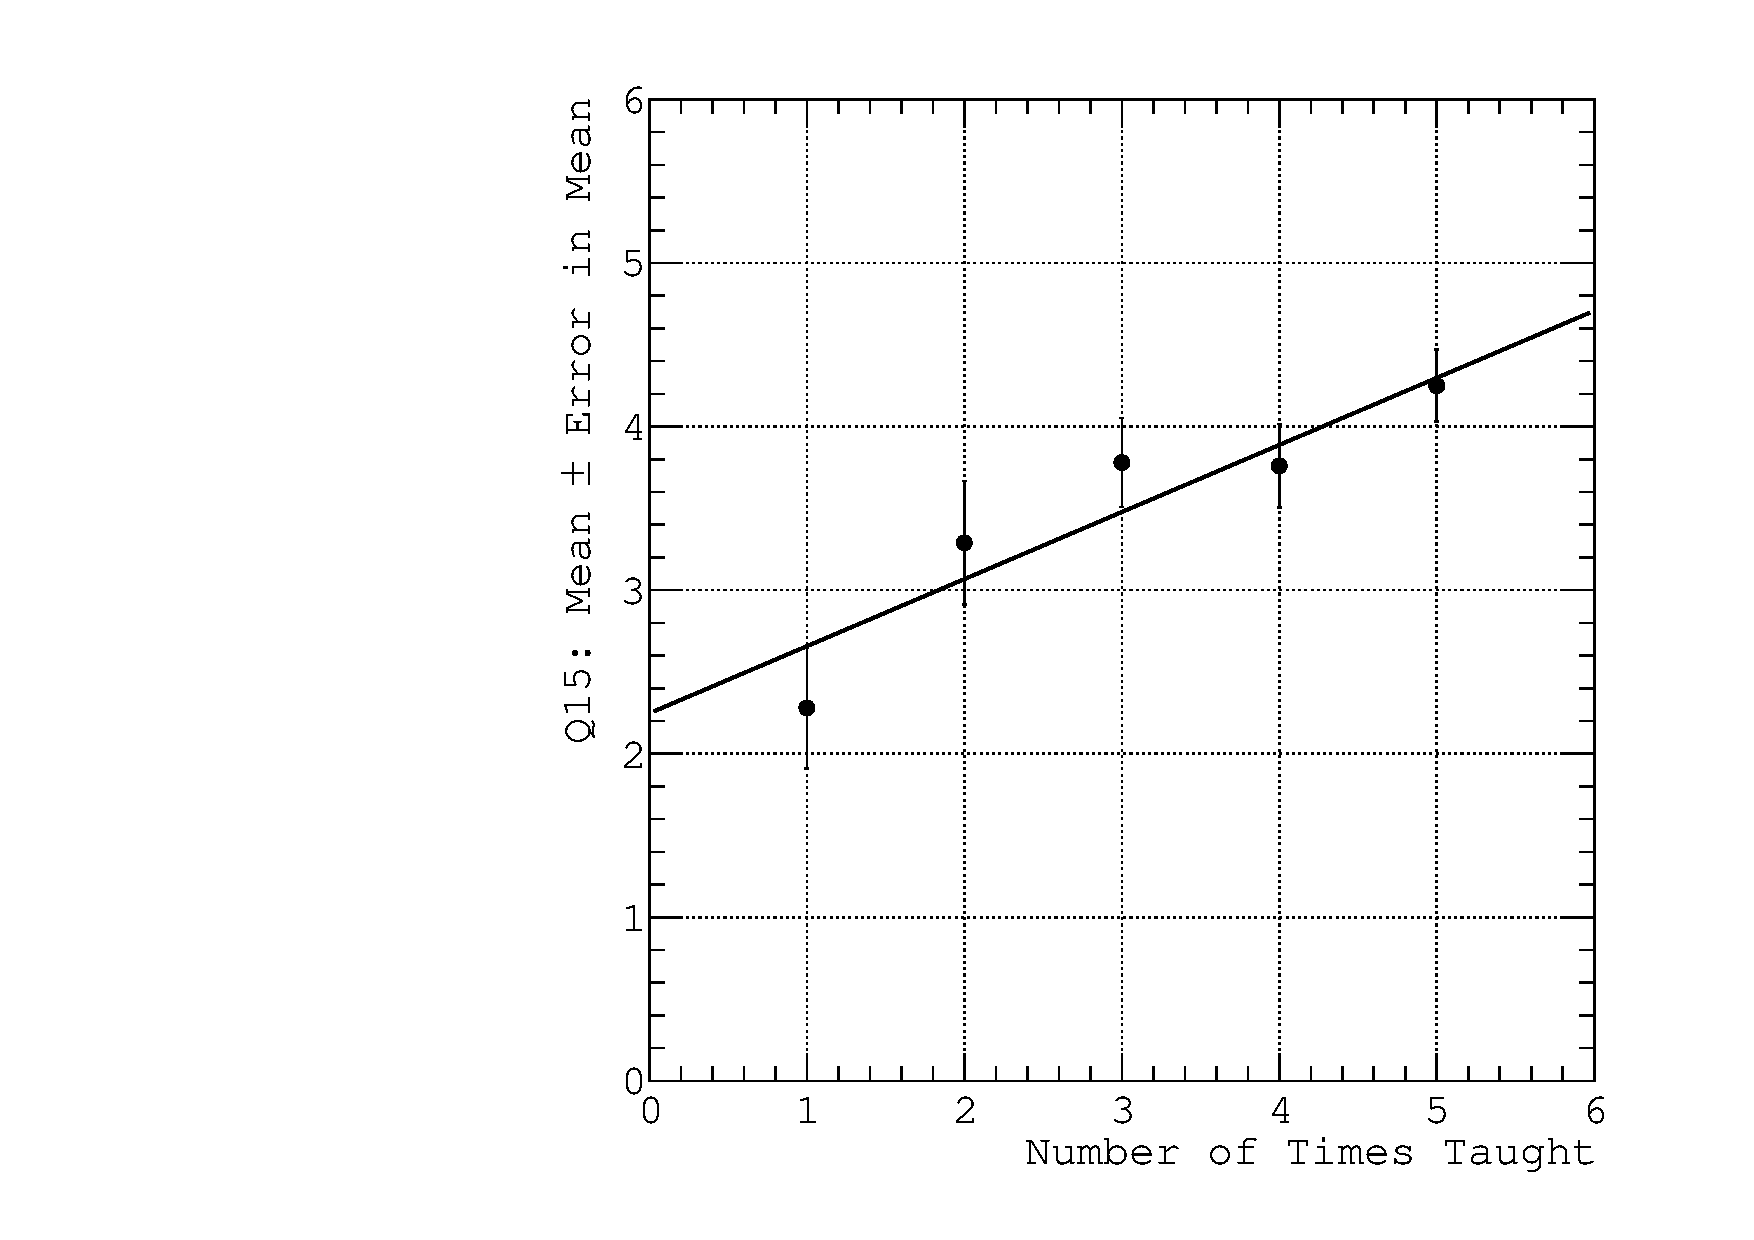
\includegraphics[width=0.4\textwidth]{Q15_algebra_based.pdf}
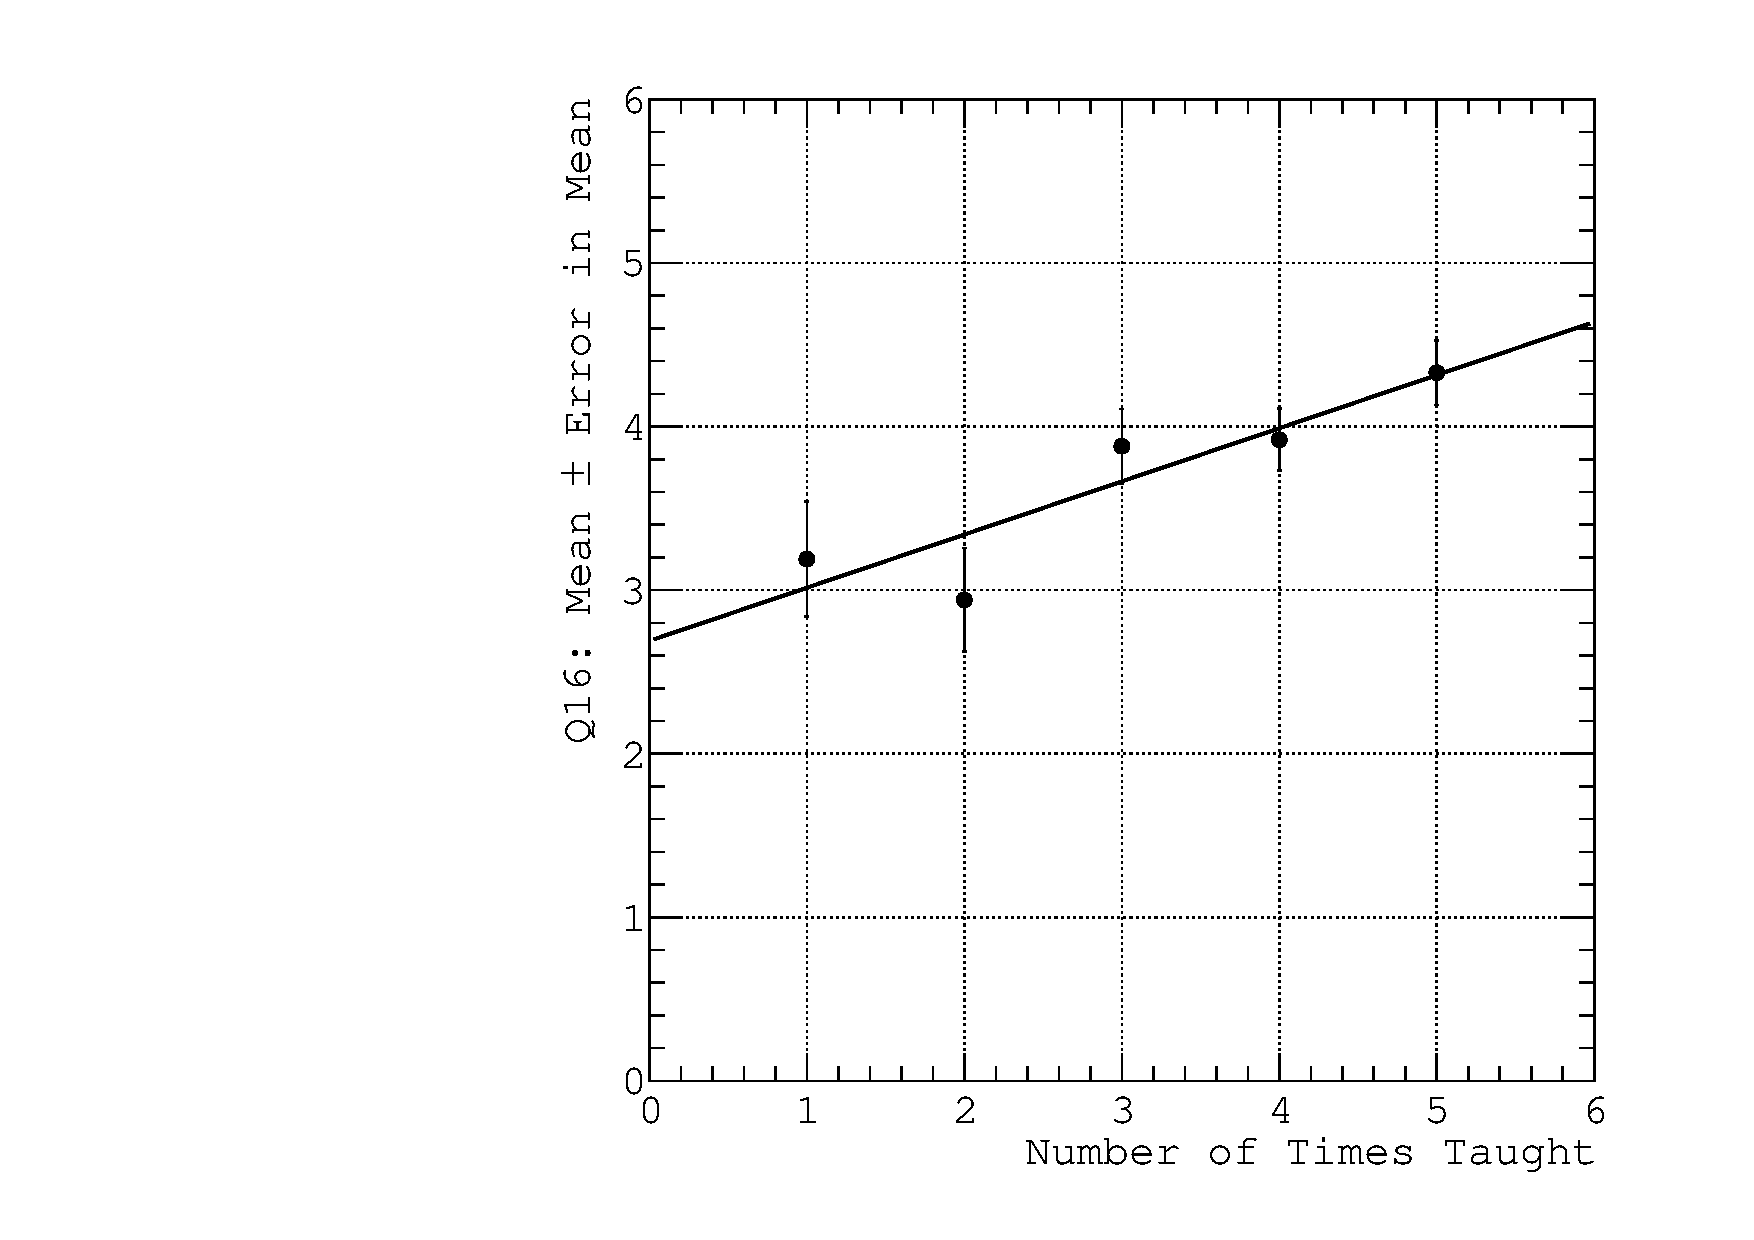
\includegraphics[width=0.4\textwidth]{Q16_algebra_based.pdf}
\caption{\label{fig:courses:intro_q15}  (Left) Student responses to Question 15 in algebra-based physics versus number of times taught. (Right) Student responses to Question 16 in algebra-based physics versus number of times taught.  The y-axis of the data points are the mean values, and the errors are the standard error in the mean.  The x-axis of the data points correspond to each time I've taught these courses.  The solid black lines are best-fit linear trend lines that minimize the $\chi^2$ value.}
\end{figure}

First, the pace of my algebra-based courses had to be slowed.  Second, I needed to include more step-by-step example problems.  Third, I needed to include more traditional lecture content.  Although one outcome is that the students reported a decrease in course difficulty (Question 11 in Tab. \ref{tab:courses:intro_shifts_1}), the most recent mean value was still $4.46 \pm 0.159$.  When I began to put these three changes in place, some students expressed such a general sense of relief that they told me in person.  One student joked that ``You could be an online professor for Chegg.com!'' He was complimenting my style by referencing a website in which instructors specialize in demonstrating solutions to common physics problems in step-by-step traditional style (similar to Khan Academy).  Struggling students copy the examples verbatim and compare new problems to these examples for reference, so beginning class with slowly worked examples appears to be the best way to establish a reference point on which students may fall back if they don't understand something.  As I've learned recently, teaching with this type of structure is especially helpful when trying to create more \textbf{inclusive classrooms} \cite{inclusive}. The simple class structure of 1) traditional content introducing concept 2) slow step-by-step example 3) PI module 4) laboratory activity/PhET seems to be the most inclusive and help the most number of students learn.  \\ \hspace{0.1cm}

Two additional comments are relevant regarding the pace of the introductory courses.  First, I chose not to reduce the number of textbook chapters covered in PHYS135A/B.  However, through attending the classes taught by Professor Zorba and Professor Lagan, I obtained a better sense of \textit{how much} content within each chapter is covered.  Drs. Zorba and Lagan have been very helpful in demonstrating how a slow and methodical lecture on a single physics topic is better retained and appreciated by the students than a faster lecture on several topics.  Professor Piner has also attended lectures in my recent classes and offered useful and positive feedback.  Second, we removed the topic of physical oscillations from PHYS150, and thermodynamics and optics from PHYS180.  In the past, PHYS180 was a 5.0 credit course because of the sheer volume of content.  In the 2018-2019 we as a department decided to create a calculus-based physics III called PHYS185 which now contains the thermodynamics, oscillations, and optics topics.  The advantage is that the pace of PHYS180 is naturally reduced by four chapters, from 15 to 11.  By taking these two major actions, my department and I are working together to accommodate the needs of our students. \\ \hspace{0.1cm}

\begin{figure}[hb]
\centering
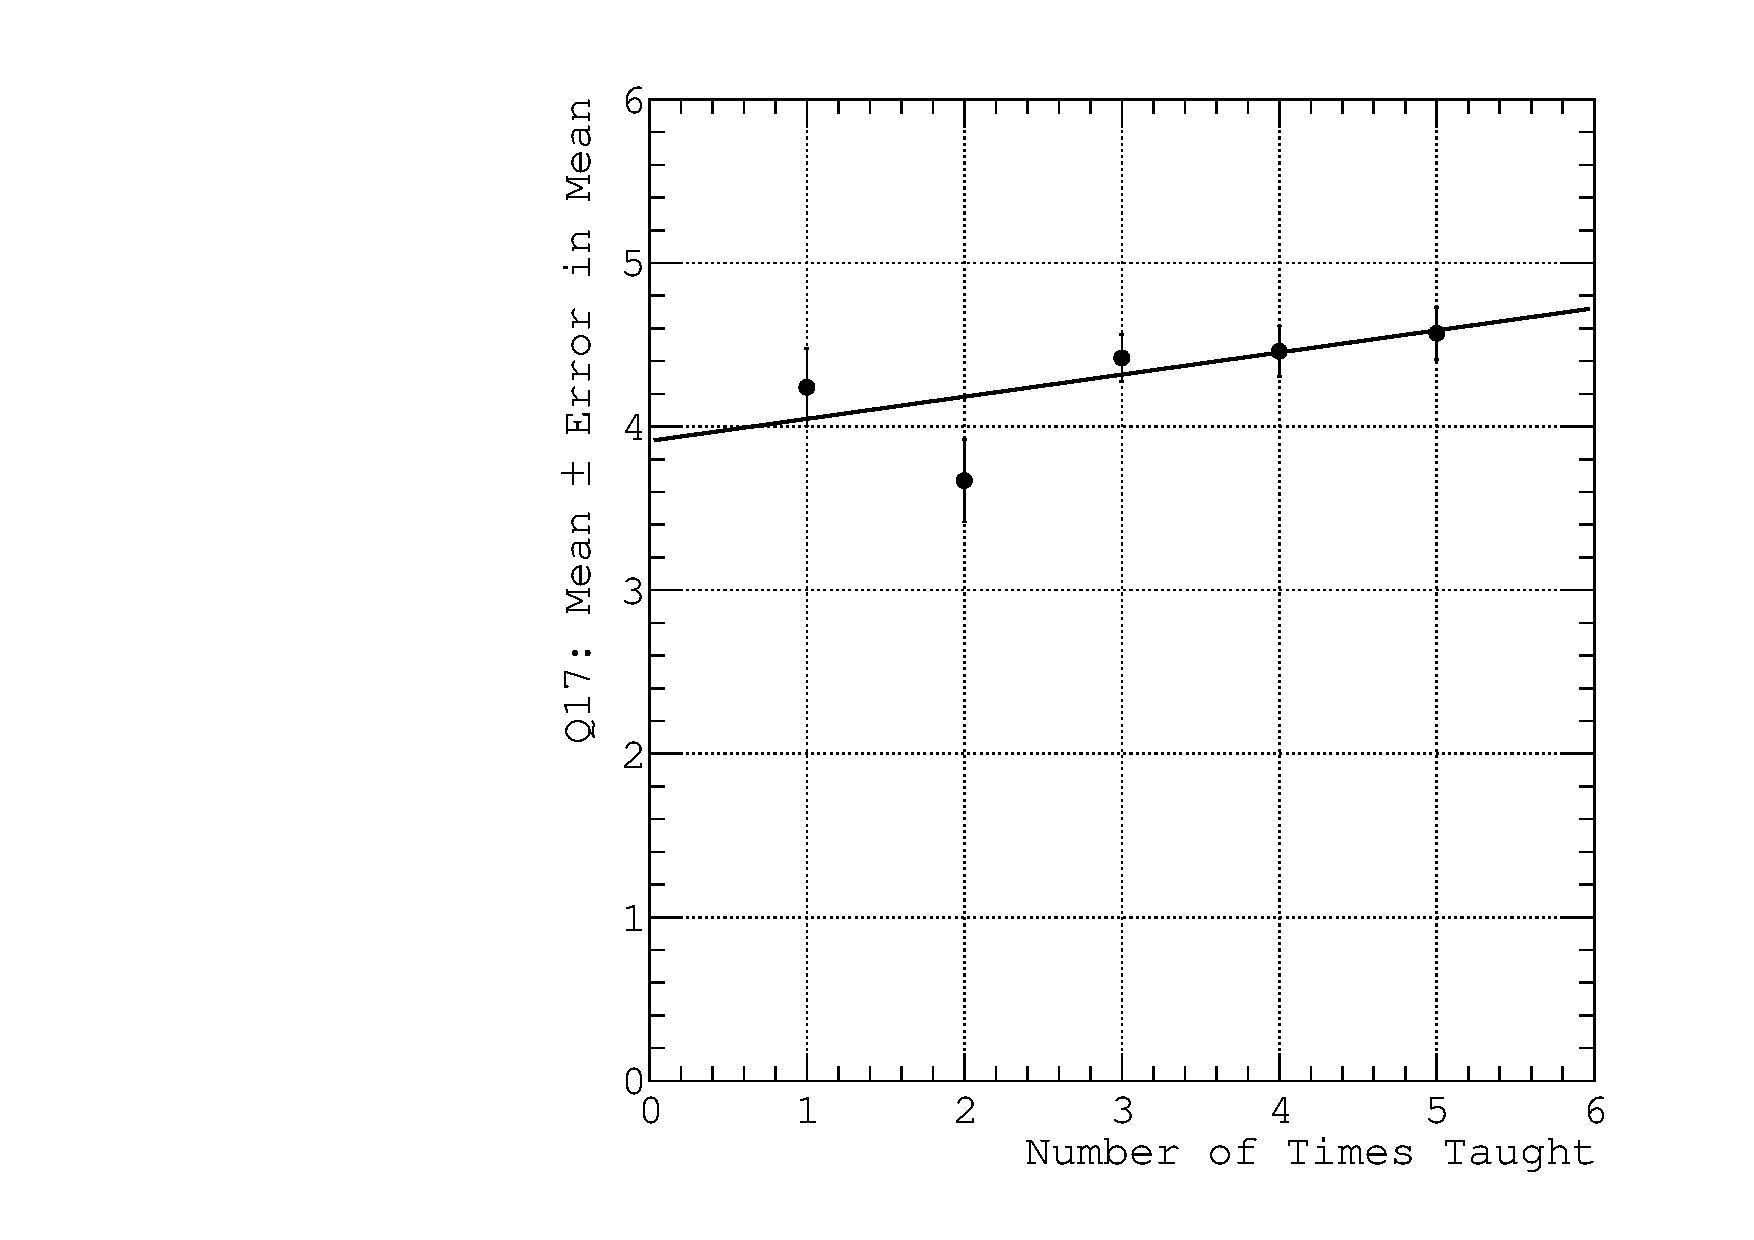
\includegraphics[width=0.4\textwidth]{Q17_algebra_based.pdf}
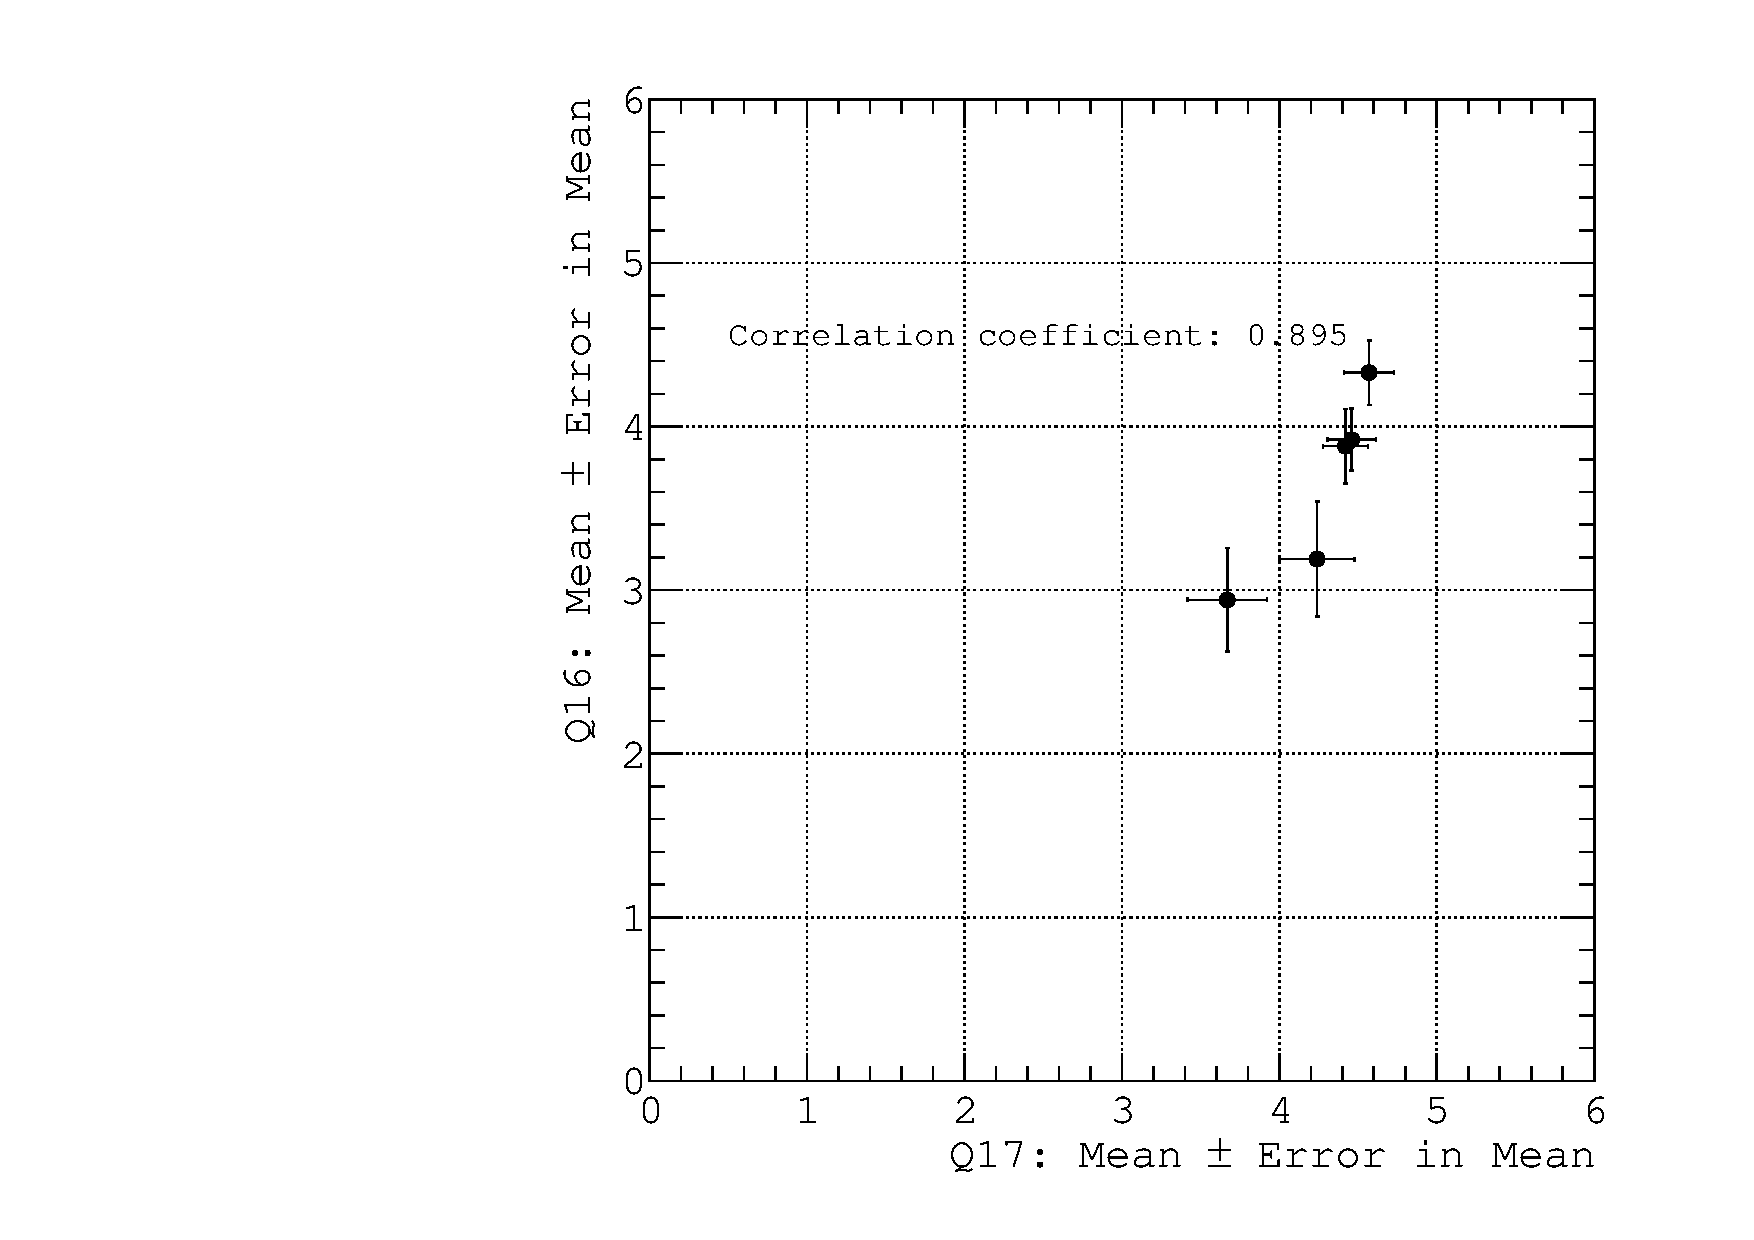
\includegraphics[width=0.4\textwidth]{Q16_Q17_algebra_based.pdf}
\caption{\label{fig:courses:intro_q17}  (Left) Student responses (mean values and errors in the mean) to Question 17 in algebra-based physics versus number of times taught. (Right) Student responses to Question 16 in algebra-based physics versus responses to Question 17.  The x and y-axis values of the data points are the mean values, and the errors are the errors in the mean.}
\end{figure}

My department also recommended that I focus on Question 17 mean values\footnote{``The professor used class time effectively and demonstrated preparation for class''.}.  Data regarding Question 17 is shown in Fig. \ref{fig:courses:intro_q17}.  My department suggested that this measurement is correlated with other key measurements like Question 16.  Figure \ref{fig:courses:intro_q17} (right) contains data suggesting this correlation is strong.  The Pearson correlation coefficient is 0.895.  In my experience, the JITT modules did not work well, and probably contributed to lower Question 17 mean values in Spring 2018 (x-value of 2 in Fig. \ref{fig:courses:intro_q17}, left).  Although I implemented them as prescribed at the 2017 AAPT workshop for new professors, the students felt they were not an effective use of class time.  These modules involve the students responding to questions assigned 1 day before class and analyzing their answers in class.  I would attempt to modify class content based on their answers in order to help the struggling students.  However, it was common for struggling students to not respond rather than risk sending me wrong answers.  This is despite the fact that I assured them they received points for completion, not accuracy.  Thus, It was difficult therefore to modify the upcoming content.  I have subsequently replaced JITT modules with traditional content and step-by-step examples.  \\ \hspace{0.1cm}

Finally, I am thrilled to report an increase in student responses to Question 25\footnote{``Overall, I would recommend this professor to others.''}. \textbf{Figure \ref{fig:courses:intro_q25} contains Question 25 mean values over time, and the data show an unmistakable and significant improvement.}  By thoughtfully implementing the changes recommended to me by my department and FPC, I see in the data that the students are endorsing me as their professor at increasing mean values over time.  I have found upon reflecting on algebra-based physics methods, that the final piece of the puzzle was to \textit{build relationships} with the students.  What follows are anecdotal stories from algebra-based classes that illustrate what I was able to accomplish by building relationships with students who needed help with a difficult subject.  \\ \hspace{0.1cm}

%Make sure to explicitly related their increased interest to the curiosity learning focus, and their increased assessment of the course to problem solving, etc.  Learning focuses.

\subsection{Anecdotes from Class, Relationships with Students}

My first story involves a senior Kinesiology major named LaJana Morris.  LaJana found the courage to approach me during the test, and ask a question about a problem.  The exercise required the students to write an equation based on the words, and solve for the missing variable $x$.  It appeared that LaJana was close to forming the correct equation, and I asked her to think conceptually about which equation from her equation sheet she should be trying to deploy.  Eventually she chose the correct one, based on the context.  I assumed she'd be able to finish, given that the problem was now reduced to solving for $x$.  I will never forget her next words: ``How do I move $x$ to get it by itself, without plugging in numbers?''  I was shocked and disappointed as I began to realize LaJana was \textit{unfamiliar with the concept of algebra.}  Of course I did not blame the student, but the question in my mind was: ``Who allowed this to happen?''  I reminded myself that my feelings were not relevant, and that I had to get the job done here.  I made it my personal mission to ensure that LaJana passed my class, and she did.  Her midterm grades improved, and by the end of the course we were both pleased.  \\ \hspace{0.1cm} %Maybe look up her grade?

My second story involves a senior WSP major named Jasmine Cao.  Jasmine is an example of an excellent student who intends to apply to medical school. \\ \hspace{0.1cm}

My third story involves a senior Biology major named Daniel Diaz.  I identified Daniel someone struggling with the material during my PI discussion rounds.

\begin{figure}
\centering
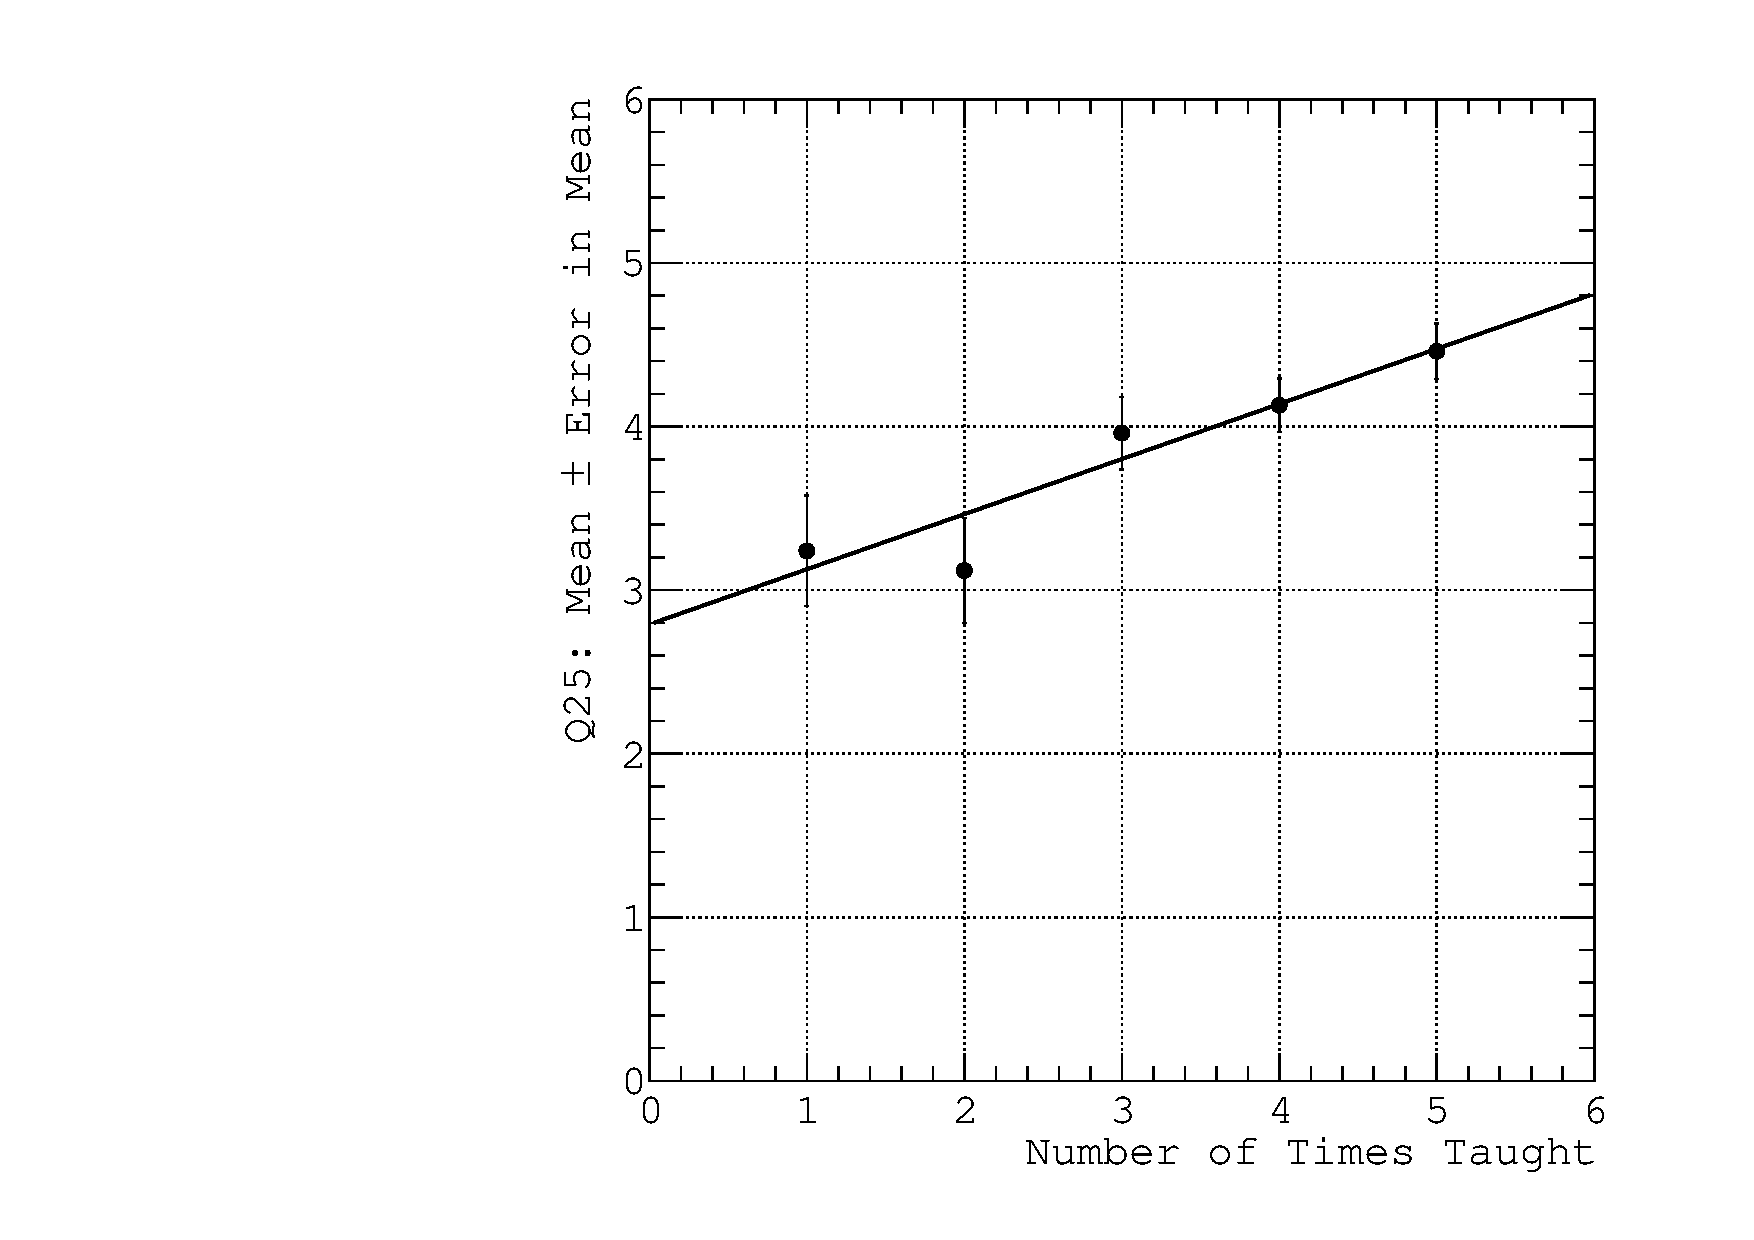
\includegraphics[width=0.4\textwidth]{Q25_algebra_based.pdf}
\caption{\label{fig:courses:intro_q25}  Student responses (mean values and errors in the mean) to Question 25 in algebra-based physics versus number of times taught.  The solid black lines are best-fit linear trend lines that minimize the $\chi^2$ value.}
\end{figure}

\begin{table}
\small
\centering
\begin{tabular}{| c | c | c |}
\hline \hline
Question & 180-02 $N$ & 180-02 result \\ \hline
10 & 8 & $5.00\pm 0.00$ \\ \hline
11 & 8 & $5.00\pm 0.00$ \\ \hline
12 & 8 & $5.00\pm 0.00$ \\ \hline
13 & 8 & $5.00\pm 0.00$ \\ \hline
14 & 8 & $5.00\pm 0.00$ \\ \hline
15 & 8 & $5.00\pm 0.00$ \\ \hline
16 & 8 & $5.00\pm 0.00$ \\ \hline
\hline
\end{tabular}
\quad
\begin{tabular}{| c | c | c |}
\hline \hline
Question & 180-02 $N$ & 180-02 result \\ \hline
17 & 8 & $5.00\pm 0.00$ \\ \hline
18 & 8 & $5.00\pm 0.00$ \\ \hline
19 & 8 & $5.00\pm 0.00$ \\ \hline
20 & 8 & $5.00\pm 0.00$ \\ \hline
21 & 8 & $5.00\pm 0.00$ \\ \hline
22 & 8 & $4.75\pm 0.25$ \\ \hline
23 & 8 & $5.00\pm 0.00$ \\ \hline
24 & 8 & $5.00\pm 0.00$ \\ \hline
25 & 8 & $5.00\pm 0.00$ \\ \hline
\hline
\end{tabular}
\caption{\label{tab:courses:intro_eval_3} (Left) Mean and error in the mean for questions 10-16 on the student evaluation form, for PHYS180-02, taught in Spring 2019.  These questions pertain to the \textit{course}.  (Right) Mean and error in the mean for questions 17-25 on the student evaluation form, for PHYS180-02, taught in Spring 2019.  These questions pertain to the \textit{professor}.}
\end{table}

\begin{table}
\small
\centering
\begin{tabular}{| c | c | c | c | c |}
\hline
\hline
Question & First Time & Most Recent Time & Raw change & Standard deviations \\
\hline
10 & 4.19 $\pm$ 0.207 & 5 $\pm$ 0 & 0.81 $\pm$ 0.207 & 3.9 \\ \hline
11 & 4.19 $\pm$ 0.345 & 5 $\pm$ 0 & 0.81 $\pm$ 0.345 & 2.35 \\ \hline
12 & 3.63 $\pm$ 0.327 & 5 $\pm$ 0 & 1.37 $\pm$ 0.327 & 4.18 \\ \hline
13 & 4 $\pm$ 0.275 & 5 $\pm$ 0 & 1 $\pm$ 0.275 & 3.64 \\ \hline
14 & 3.93 $\pm$ 0.333 & 5 $\pm$ 0 & 1.07 $\pm$ 0.333 & 3.22 \\ \hline
15 & 3.56 $\pm$ 0.315 & 5 $\pm$ 0 & 1.44 $\pm$ 0.315 & 4.57 \\ \hline
16 & 3.56 $\pm$ 0.315 & 5 $\pm$ 0 & 1.44 $\pm$ 0.315 & 4.57 \\ \hline
17 & 3.31 $\pm$ 0.285 & 5 $\pm$ 0 & 1.69 $\pm$ 0.285 & 5.93 \\ \hline
18 & 2.88 $\pm$ 0.34 & 5 $\pm$ 0 & 2.12 $\pm$ 0.34 & 6.24 \\ \hline
19 & 3.13 $\pm$ 0.385 & 5 $\pm$ 0 & 1.87 $\pm$ 0.385 & 4.86 \\ \hline
20 & 3.69 $\pm$ 0.312 & 5 $\pm$ 0 & 1.31 $\pm$ 0.312 & 4.19 \\ \hline
21 & 3.88 $\pm$ 0.273 & 5 $\pm$ 0 & 1.12 $\pm$ 0.273 & 4.11 \\ \hline
22 & 3.81 $\pm$ 0.333 & 4.75 $\pm$ 0.251 & 0.94 $\pm$ 0.417 & 2.26 \\ \hline
23 & 3.67 $\pm$ 0.343 & 5 $\pm$ 0 & 1.33 $\pm$ 0.343 & 3.88 \\ \hline
24 & 4.5 $\pm$ 0.157 & 5 $\pm$ 0 & 0.5 $\pm$ 0.157 & 3.17 \\ \hline
25 & 3.13 $\pm$ 0.407 & 5 $\pm$ 0 & 1.87 $\pm$ 0.407 & 4.59 \\ \hline
\hline
\end{tabular}
\caption{\label{tab:courses:intro_shifts_2} Comparison calculus-based numbers for the first time taught (first column) to the most recent time (second column). The raw change is given in the third column, and the change divided by the standard deviation is given in the fourth column.}
\end{table}

%In \textit{calculus-based physics}, the story was different.  There are many areas in which the courses and my teaching scored well.  \textbf{I am especially proud of the fact that Q25 (``Overall, I would recommend this professor to others'') jumped in 2018 relative to 2017 for the calculus-based courses.  In fact, my teaching scores improved in almost every category in calculus-based physics in going from Fall 2017 to Spring 2018.}  Further, students in both sections believed that the courses were rigorous and challenging, while still giving me increasing marks in all categories.  Some students appreciated the PI modules, PhET simulations, and JITT exercises.  This is reflected in responses to question 12 on the standard evaluation (``This course offered useful learning tools''), which is a key data point.  I focus on this data point because I am being asked by my department to teach in an activities based style with modules like PI-modules, different from the traditional lecture.  The purpose of the activities and group exercises is to satisfy the focus on \textbf{improvement of analysis skill}.  The PI, JITT, and PhET modules are constructed to improve analysis skill through conceptual understanding.  However, upon reflecting on the students' constructive comments, it seems that these modules benefit some students but not all. \\ \hspace{0.1cm}

%A vital teaching method emerged in PHYS180, which the students call ``board problems'' in their written responses to evaluations.  It started with an interesting compromise between my desire to move forward in the book faster, and the students' desire to go slowly and have me do examples.  Notice that in the PHYS180 written responses, the students still express quite often a desire for worked examples in class.  In light of all the research-based teaching methods that encourage students to learn through interactions with each other, I decided to have them \textit{work example problems for each other}.  I began by giving an example problem to the class.  The problem would be difficult, and I would either design it myself, or draw it from the current chapter.  Students would then work the problem in groups of 3-4 on the whiteboards, next to other groups.  The class responded positively to this method, and it is reflected in their written responses.  Some even state explicitly that my teaching improved!  The board-problem method works for two reasons: it allows struggling students to see how harder problems are approached by peers, and struggling groups see other groups' strategies and therefore learn from the whole class.  \\ \hspace{0.1cm}

%The success of the ``board problems'' technique also reflected the fact that some of the issues PHYS150/PHYS180 students shared were similar to those in PHYS135A/B.  Some students wrote that the pace was too fast, while others reminded me that this was the first time they had encountered mathematical concepts like vector fields.  Students also wrote that class time should be used more effectively, with fewer PhET simulations and more concrete traditional lecturing with examples.  Finally, some students wrote that they didn't benefit from the summarization of scientific articles (meant to practice scientific oral communication).  A handful of students seemed to express the opposite opinion, that there should be more of that activity.  Going forward, I have learned that inclusion of communication activities should be gauged mid-semester, and I will include them if the students are eager and if time permits.

%Having reflected extensively on all of the student feedback, I have decided on \textbf{three concrete improvements} to my introductory courses.  In consultation with my department chair, and in studying past PEGP documents in my department, the first improvement will be an increase in traditional lecture content.  The reason is that if every single concept and number in physics is confusing to a first-time student, then merely updating the teaching style with researched-based modules will not help that student.  The traditional lecture style offers the benefit that students see many example problems done in explicit detail, such that they can copy and repeat the technique.  I was taught to never expect this as an undergraduate student.  My colleagues in my department have reassured me that it is necessary to give inexperienced students an explicit starting point.  Thus, going forward in my introductory courses, \textit{a significant fraction of class-time will be spent on concrete examples in the traditional style.} \\ \hspace{0.1cm}

%The second major change I will be making to my introductory course teaching style is to slow the pace.  In reading students' remarks, this is the second most common desire on their part.  I was taught at the undergraduate and graduate levels at high speed, with intense focus on both content and mathematical detail.  Of course I must make adjustments for the environment at Whittier College, and not merely teach to myself.  I must \textit{teach to the middle}, as one of my colleagues recommended.  The students felt relief when I began assigning them board-problems, precisely because it allowed them to slow down, and check their work with each other and other groups.  Thus, the addition of board-problems solved both the problem of pace and example problems at once.  The students got a chance to lecture to each other momentarily.  In the coming semesters, \textit{I will include the group-board technique regularly}. One minor adjustment to this technique is that the courses are getting larger enrollments, and we may run out of whiteboard space.  My plan is to sketch the problem, and then allow student groups to design specific examples meant to be exchanged with another group.  This is working in my Fall 2018 PHYS135A sections when it's not feasible to do board-problems.  \\ \hspace{0.1cm}

%The third change I'd like to make is to include more applications of calculus in the \textit{calculus-based} introductory sequences.  In my view, more applications of calculus should be included in PHYS150/PHYS180.  From the feedback from my department, I need to include more laboratory activities in PHYS180.  Thus, I propose solving both problems simultaneously.  When I teach \textit{calculus-based} introductory courses in the future, I will use the laboratory activities as a venue for demonstrating the difference between results obtained with and without calculus.  The inclusion of more lab activities is mandatory (and now possible because I'm fully trained on all the equipment).  Thus including calculus concepts in the labs will require little extra effort.  Finally, homework problems involving calculus will be selected from the book's less-difficult category, easing the transition from math to physics contexts. \\ \hspace{0.1cm}

%In consultation with my department, I have been focusing on question 17 (``The professor used class time effectively and demonstrated preparation for class.'').  My colleagues believe that many numbers will rise in correlation with question 17.  Struggling students who desired traditional lectures with examples and worksheets likely felt class was not organized because they were unaccustomed to research-based modules like PI or PhET.  Of course I prepared for my courses; I have built an interactive, open-source GB-scale database of lecture content \footnote{see my account on Github.com: \url{https://github.com/918particle/AlgebraBasedMechanics1} or \url{https://github.com/918particle/AlgebraBasedMechanics1}.}.  Going forward, I can use the discussion period during PI modules to focus on helping struggling students one-on-one with a mini-lecture at their table.  The group board problems also afford me the chance to do this.  Finally, providing more traditional lecture content should help the situation. For further analysis of the data in Tab. \ref{tab:courses:intro_eval_1}-\ref{tab:courses:intro_eval_4}, see Appendix A. \\ \hspace{0.1cm}

\end{document}